\section{Heurística de Búsqueda Local}

\subsection{Algoritmo}

\begin{algorithm}[H]
\caption{} 
\begin{codebox}
\Procname{$\proc{maximoImpactoLocal}(Grafo$ g$, Grafo$ h$, double $ porcentaje$)$}

\li
\li vector$<$unsigned int$>$ impactoGoloso  $\gets$ maximoImpactoGoloso(g,h,porcentaje)
\li unsigned int impactoParcial $\gets$ impactoGoloso[0];
\li vector$<$unsigned int$>$ coloreo(n);
\li
\li \For i desde 1 hasta n \Do
    
\li 	coloreo[i] $\gets$ impactoGoloso[i]
    
    \End
\li

\li unsigned int nuevoImpacto $\gets$ 0
\li
\li	\For i desde 1 hasta n \Do
	
\li
\li		vector$<$unsigned int$>$ vecinos $\gets$ $vecinos del nodo i en h$
\li
\li 	\For j desde 1 hasta la cantidad de vecinos de i en h \Do

\li				unsigned int color = coloreo[vecinos[j]]
\li
\li				\If pintar al nodo i de $color$ es legal \Do			
\li						vector$<$unsigned int$>$ nuevoColoreo $\gets$ \quad $coloreo$
\li						nuevoColoreo[i]$ \gets$ \quad $color$
\li                		nuevoImpacto $ \gets$ \quad $h.impacto(nuevoColoreo)$
\li
\li                		\If nuevoImpacto $>$ impactoParcial \Do
                
\li                			coloreo[i] $\gets$ \quad $color$
\li                   			impactoParcial $\gets$ \quad $nuevoImpacto$
                   		\End
\li
                \End
        \End
    \End

\li
\li		impactoGoloso[0] $\gets$ \quad $impactoParcial$
\li
\li \For i desde 0 hasta n \Do
\li		impactoGoloso[i+1]=coloreo[i]
	\End    

\li
\li return impactoGoloso
\End
\end{codebox}
\end{algorithm}

\subsection{Análisis de complejidad}

\indent Veamos la complejidad de maximoImpactoLocal. Primero se calcula una solución con maximoImpactoGoloso. Como mencionamos en el apartado correspondiente eso cuesta O(n*(n+m)+ $n^{3}$). \\
\indent Luego, se copia el coloreo que se obtuvo de maximoImpactoGoloso en O(n).\\
\indent A continuación se itera sobre la cantidad de nodos de H. En cada iteración se copian los vecinos del nodo en el que estamos ahora. Como dicho nodo puede tener a lo sumo n-1 vecinos, eso cuesta O(n). Luego,se itera sobre los vecinos del nodo y por cada vecino del nodo se decide en O(n+m) si se va a pintar el nodo del mismo color que su vecino. Dicha decisión se fundamenta en si cambiar el color genera un coloreo válido en G y si aumenta el impacto H. Entonces,el costo del ciclo interior cuesta O(n*(n+m)). Por lo tanto, el ciclo que lo engloba cuesta O($n^{2}$*(n+m)).\\
\indent Luego de terminar de iterar se guarda el coloreo parcial con un costo de O(n).\\
\indent Entonces, maximoImpactoLocal cuesta O(n*(n+m)+ $n^{3}$ +$ n^{2}$*(n+m)).\\

\subsection{Experimentación y Resultados}
\quad Trabajamos con los siguientes 3 casos: grafos al azar, grafos densos, G y H complementos.

\quad Se midieron los tiempos en corridas de  5 a 100 nodos con 100 repeticiones para cada cantidad de nodos.

\subsubsection{Grafos al azar}

\begin{figure}[H]
	\centering
	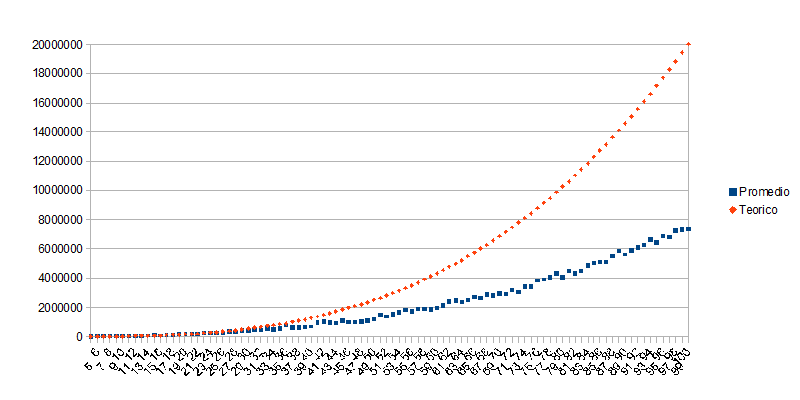
\includegraphics[scale=0.8]{BLocal-tiempos-Azar.png}
\caption{Costos}
\end{figure}

\subsubsection{Grafos densos}

\begin{figure}[H]
	\centering
	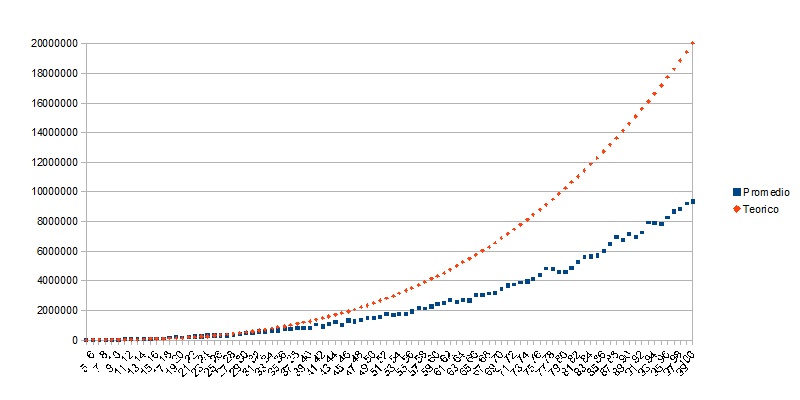
\includegraphics[scale=0.8]{BLocal-tiempos-G-y-H-densos.png}
\caption{Costos}
\end{figure}

\subsubsection{G y H complementos}

\begin{figure}[H]
	\centering
	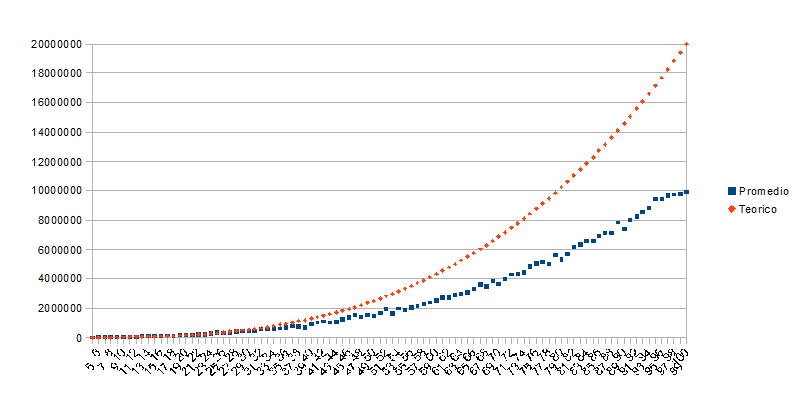
\includegraphics[scale=0.8]{BLocal-tiempos-H-complemento.png}
\caption{Costos}
\end{figure}